\documentclass[UTF8,12pt]{article} % 12pt 为字号大小
\usepackage{amssymb,amsfonts,amsthm}
%\usepackage{fontspec,xltxtra,xunicode}
%\usepackage{times}
\usepackage{amsmath,bm}
\usepackage{mdwlist}
\usepackage[colorlinks,linkcolor=blue]{hyperref}
\usepackage{cleveref}
\usepackage{float}
\usepackage{enumerate}
\usepackage{extarrows}


%----------
% 定义中文环境
%----------

\usepackage{xeCJK}
\setCJKmainfont[BoldFont={Heiti SC Light},ItalicFont={Kaiti SC Regular}]{Songti SC Regular}
\setCJKsansfont{Heiti SC Light}
\setCJKfamilyfont{song}{Songti SC Regular}
\setCJKfamilyfont{zhhei}{Heiti SC Light}
\setCJKfamilyfont{zhkai}{Kaiti SC Regular}
\setCJKfamilyfont{zhfs}{STFangsong}
\setCJKfamilyfont{zhli}{Libian SC Regular}
\setCJKfamilyfont{zhyou}{Yuanti SC Regular}

\newcommand*{\songti}{\CJKfamily{zhsong}} % 宋体
\newcommand*{\heiti}{\CJKfamily{zhhei}}   % 黑体
\newcommand*{\kaiti}{\CJKfamily{zhkai}}  % 楷体
\newcommand*{\fangsong}{\CJKfamily{zhfs}} % 仿宋
\newcommand*{\lishu}{\CJKfamily{zhli}}    % 隶书
\newcommand*{\yuanti}{\CJKfamily{zhyou}} % 圆体

%----------
% 版面设置
%----------
%首段缩进
\usepackage{indentfirst}
\setlength{\parindent}{2em}

%行距
\renewcommand{\baselinestretch}{1.2} % 1.2倍行距

%页边距
\usepackage[a4paper]{geometry}
\geometry{verbose,
  tmargin=2cm,% 上边距
  bmargin=2cm,% 下边距
  lmargin=2.5cm,% 左边距
  rmargin=2.5cm % 右边距
}


%----------
% 其他宏包
%----------
%图形相关
\usepackage[x11names]{xcolor} % must before tikz, x11names defines RoyalBlue3
\usepackage{graphicx}
\graphicspath{{figures/}}
\usepackage{pstricks,pst-plot,pst-eps}
\usepackage{subfig}
\def\pgfsysdriver{pgfsys-dvipdfmx.def} % put before tikz
\usepackage{tikz}

%原文照排
\usepackage{verbatim}

%网址
\usepackage{url}

%----------
% 定理、习题与解答环境
%----------
%定理环境
\usepackage[most]{tcolorbox}
\newtcbtheorem[number within=section]{theorem}{Theorem}{
     enhanced,
     breakable,
     sharp corners,
     attach boxed title to top left={
       yshifttext=-1mm
     },
     colback=white,
     colframe=blue!75!black,
     fonttitle=\bfseries,
     boxed title style={
       sharp corners,
       size=small,
       colback=blue!75!black,
       colframe=blue!75!black,
     } 
}{theorem}

\newtcbtheorem[number within=section]{definition}{Definition}{
     enhanced,
     breakable,
     sharp corners,
     attach boxed title to top left={
       yshifttext=-1mm
     },
     colback=white,
     colframe=blue!75!black,
     fonttitle=\bfseries,
     boxed title style={
       sharp corners,
       size=small,
       colback=blue!75!black,
       colframe=blue!75!black,
     } 
}{definition}

\newtcbtheorem[number within=section]{corollary}{Corollary}{
     enhanced,
     breakable,
     sharp corners,
     attach boxed title to top left={
       yshifttext=-1mm
     },
     colback=white,
     colframe=blue!75!black,
     fonttitle=\bfseries,
     boxed title style={
       sharp corners,
       size=small,
       colback=blue!75!black,
       colframe=blue!75!black,
     } 
}{corollary}

\newtcbtheorem[number within=section]{myboxes}{Box}{
     enhanced,
     breakable,
     sharp corners,
     attach boxed title to top left={
       yshifttext=-1mm
     },
     %colback=white,
     colframe=black!75!white,
     fonttitle=\bfseries,
     boxed title style={
       sharp corners,
       size=small,
       colback=black!75!white,
       colframe=black!75!white,
     } 
}{myboxes}

%习题环境
\newtcbtheorem[number within=section]{exercise}{Problem}{
     enhanced,
     breakable,
     sharp corners,
     attach boxed title to top left={
       yshifttext=-1mm
     },
     colback=white,
     colframe=black,
     fonttitle=\bfseries,
     boxed title style={
       sharp corners,
       size=small,
       colback=black,
       colframe=black,
     } 
}{Problem}

%解答环境
\ifx\proof\undefined\
\newenvironment{proof}[1][\protect\proofname]{\par
\normalfont\topsep6\p@\@plus6\p@\relax
\trivlist
\itemindent\parindent
\item[\hskip\labelsep
\scshape
#1]\ignorespaces
}{%
\endtrivlist\@endpefalse
}
\fi

\renewcommand{\proofname}{\it{Solution}}



%==========
% 正文部分
%==========

\begin{document}

\title{Chapter 2}
\author{Yuquan Chen}
\date{2019/03/19} % 若不需要自动插入日期,则去掉前面的注释;{ } 中也可以自定义日期格式
\maketitle

\section{Time evolution operator and Hamiltonian}

Here, we talk about non-relativistic situation, and we think about time as a parameter, not an operator. The position representation $\langle x|\psi\rangle = \psi(x)$, adding the time evolution, we have $$\langle x|\psi(t)\rangle = \psi(x,t)$$
First, we talk about 6 postulates of quantum mechanics.\\

\begin{myboxes}{Postulates of Quantum Mechanics}{}
\textbf{Postulate 1.} At any time $t$, the state of a physical system is defined by a ket $|\psi\rangle$, or \textit{state} in a relevant Hilbert space $H$.\\\par
\textbf{Postulate 2.} The only possible result of measuring observable $A$ is one of the eigenvalues of $A$
\begin{figure}[H]
\begin{center}
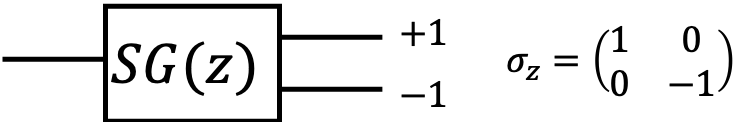
\includegraphics[width=7cm]{post2}
%\caption{}
%\label{}
\end{center}
\end{figure}
Aside:
\begin{enumerate*}
\item If $A$ is Hermitian, then the measurement gives a real number.
\item If $A$'s spectrum is discrete, then we only see quantized result.
\end{enumerate*}
\textbf{Postulate 3.} Every measurable physical quantity $A$ is described by a Hermitian operator.\\\par
\textbf{Postulate 4.} If $A|u_{\alpha}\rangle = a_{\alpha}|u_{\alpha}\rangle$, then for a system in $|\psi\rangle$, when we measure $A$, then the probability of getting $a_{\alpha}$ is $P(a_{\alpha}) = |\langle u_{\alpha}|\psi\rangle|^{2}$.\\
Aside: If we have degenerate $a_{\alpha}$'s $\{|u_{\alpha,1}\rangle, |u_{\alpha,2}\rangle, ...\}$ share the same eigenvalue, then $P(a_{\alpha}) = \sum_{i} |\langle u_{\alpha,i}|\psi\rangle|^{2}$\\
Example: $A = I$, all $a_{\alpha} = 1$\\\par
\textbf{Postulate 5.} If a measurement projects $|\psi\rangle$ into a new state $|u_{\alpha}\rangle$, then a physical new state should be $|u_{\alpha}'\rangle = \frac{|u_{\alpha}\rangle}{\sqrt{\langle u_{\alpha}|u_{\alpha}\rangle}}$, so that $\langle u_{\alpha}'|u_{\alpha}'\rangle = 1$.\\\par
\textbf{Postulate 6.} Between measurement the state vector $|\psi(t)\rangle$ evolves in time with time dependent Shr\"{o}dinger's equation $$i\hbar \frac{d}{dt}|\psi(t)\rangle = \hat{H}(t)|\psi(t)\rangle$$ here $\hat{H}$ is a Hamiltonian.
\end{myboxes}

We let a displacement $dt'$ on state $|\psi(t)\rangle$,
\begin{align}\label{dt}
\Rightarrow U(dt')|\psi(t)\rangle = |\psi(t+dt')\rangle,~\text{where } UU^{\dag} = 1
\end{align}
It's similar to momentum, in that case, we have
$$\begin{cases}U(dt') = I - i\frac{\hat{H}}{\hbar}dt'\\\hat{H} \text{ is Hermitian, called Hamiltonian}\end{cases}$$
so (\ref{dt}) could be evaluated as:
\begin{align}
\text{LHS} &= \left(I - i\frac{\hat{H}}{\hbar}dt'\right) \psi(x,t) = \psi(x,t) -  i\frac{\hat{H}}{\hbar}dt'\psi(x,t) \\
\text{RHS} &= \psi(x,t+dt') = \psi(x,t) + \left(\frac{\partial}{\partial t}\psi(x,t)\right)dt'
\end{align}
\begin{align}
\Rightarrow \boxed{i\hbar\frac{\partial}{\partial t} \psi(x,t) = H\psi(x,t)}
\end{align}
which is Shr\"{o}dinger's equation in position representation. In general, we have
\begin{align}\label{shordinger}
\boxed{i\hbar\frac{\partial}{\partial t} |\psi(t)\rangle = H|\psi(t)\rangle}
\end{align}
$H$: Hamiltonian in analog to classical mechanics,
\begin{align}
H = T + V,~ \begin{cases}T = \frac{p^{2}}{2m} \text{ is kinetic energy} \\ V \text{ is potential energy}\end{cases}
\end{align}
and in quantum mechanics, we have
\begin{align}
\hat{H} = \hat{T} + \hat{V} = \frac{\hat{p}^{2}}{2m} + \hat{V}(x)
\end{align}

Here are some examples of Hamiltonians in different systems.

\begin{myboxes}{Examples of Hamiltonians in different systems}{}
\begin{enumerate*}
\item A free particle $V=0$ $$\hat{H} = \frac{\hat{p}^{2}}{2m}$$
\item Hydrogen atom $$\hat{H} = \frac{\hat{p}_{e}^{2}}{2m_{e}} + \frac{\hat{p}_{n}^{2}}{2m_{n}} - \frac{e^{2}}{4\pi\varepsilon_{0}|\vec{r}_{e}-\vec{r}_{n}|}$$
\item A particle with magnetic momentum $\vec{\mu}$, in external magnetic field $\vec{B}$
$$\hat{H} = -\vec{\mu}\cdot\vec{B}$$
\end{enumerate*}
\end{myboxes}

As $\hat{H} = \frac{\hat{p}^{2}}{2m}$, it's convenient to work in momentum representation $\{|p\rangle\}$ as our basis. We apply $\langle p|$ on the left of equation $H|\psi(t)\rangle = i\hbar\frac{\partial}{\partial t}|\psi(t)\rangle$, we get
\begin{align}
&\text{LHS} = \left(\langle p|\frac{\hat{p}^{2}}{2m}\right)|\psi(t)\rangle = \frac{p^{2}}{2m} \langle p|\psi(t)\rangle = \frac{p^{2}}{2m} \psi(p,t) \\
&\text{RHS} = i\hbar\langle p|\frac{\partial}{\partial t}|\psi(t)\rangle \xlongequal{\frac{\partial}{\partial t}\langle p| = 0} i\hbar\frac{\partial}{\partial t}\langle p|\psi(t)\rangle = i\hbar\frac{\partial}{\partial t}\psi(p,t) \\
&\Rightarrow \frac{p^{2}}{2m}\psi(p,t) = i\hbar\frac{\partial}{\partial t}\psi(p,t) \\
&\Rightarrow \psi(p,t) = \psi(p,0) e^{-i\frac{p^{2}t}{2m\hbar}}
\end{align}
if we let
\begin{align}
\psi(p,0) = \frac{1}{\sqrt{2\pi\hbar}} e^{-i\frac{px}{\hbar}} \sim \langle x|p\rangle
\end{align}
in this case, 
\begin{align}
\boxed{\psi(p,t) = \frac{1}{\sqrt{2\pi\hbar}} e^{-i\frac{px}{\hbar}} e^{-i\frac{p^{2}t}{2m\hbar}} = \frac{1}{\sqrt{2\pi\hbar}} e^{-i\frac{p}{\hbar}\left(x + \frac{pt}{m}\right)}}
\end{align}
we have
\begin{align}
\psi(p,0) &= \langle p|x\rangle \text{ momentum representation of } |x\rangle \\
\psi(p,t) &= \langle p|x + \frac{pt}{m}\rangle \text{ if set } v=\frac{p}{m} \text{, then } x+\frac{pt}{m} = x+vt
\end{align}

\begin{myboxes}{Comment}{}
We should observe structure of $H$, and choose the right representations. We have
$$\psi(x,0) \xrightarrow[\text{rewrite in p-repres}]{\text{Fourier transform}} \psi(p,0)$$
$$\psi(p,t) \xlongequal{H = \frac{p^{2}}{2m}} \psi(p,0) e^{-i\frac{p^{2}t}{2m\hbar}}$$
if we need $\psi(x,t)$, we can get it from another Fourier transformation from $\psi(p,t)$.
\end{myboxes}

\section{Static Shr\"{o}dinger's equation}

Recall equation (\ref{shordinger}) that
$$\hat{H}|\psi(t)\rangle = i\hbar\frac{\partial}{\partial t}|\psi(t)\rangle$$
in position representation,
\begin{align}
\langle x|\hat{H}|\psi(t)\rangle &= i\hbar\frac{\partial}{\partial t}\langle x|\psi(t)\rangle \\
\Rightarrow H\psi(x,t) &= i\hbar\frac{\partial}{\partial t}\psi(x,t)
\end{align}
where $H = \frac{\hat{p}^{2}}{2m} + V(x),~ \hat{p} \leftrightarrow -i\hbar\frac{\partial}{\partial x}$,
\begin{align}\label{sex}
\Rightarrow \boxed{-\frac{\hbar^{2}}{2m}\frac{\partial^{2}}{\partial x^{2}}\psi(x,t) + V(x)\psi(x,t) = i\hbar\frac{\partial}{\partial t}\psi(x,t)}
\end{align}

\begin{myboxes}{A common mistake}{}
We know that in $x$ representation, $\hat{p} \leftrightarrow -i\hbar\frac{\partial}{\partial x}$, but
$$\langle x|\hat{p}^{2}|\psi\rangle \ne -\hbar^{2}\left(\frac{\partial}{\partial x} \psi(x)\right)^{2}$$
instead, 
$$\boxed{\langle x|\hat{p}^{2}|\psi\rangle = -\hbar^{2}\frac{\partial^{2}}{\partial x^{2}}\psi(x)}$$
because we have
$$\langle x|\hat{p}|\psi\rangle = -i\hbar\frac{\partial}{\partial x}\langle x|\psi\rangle = -i\hbar\frac{\partial}{\partial x}\psi(x)$$
then
\begin{align*}
\langle x|\hat{p}^{2}|\psi\rangle \xlongequal{|\phi\rangle = \hat{p}|\psi\rangle}& \langle x|\hat{p}|\phi\rangle =  -i\hbar\frac{\partial}{\partial x}\langle x|\phi\rangle = (-i\hbar)\frac{\partial}{\partial x}\langle x|\hat{p}|\psi\rangle \\
=& (-i\hbar)\frac{\partial}{\partial x}\left(-i\hbar\frac{\partial}{\partial x}\langle x|\psi\rangle\right) = -\hbar^{2}\frac{\partial}{\partial x}\left(\frac{\partial}{\partial x}\psi(x)\right) \\
=& -\hbar^{2}\frac{\partial^{2}}{\partial x^{2}}\psi(x)
\end{align*}
\end{myboxes}

To solve equation (\ref{sex}), it's best to separate the variables. Suppose we set
\begin{align}
\psi(x,t) = \Psi(x)\phi(t)
\end{align}
where $\hat{H}$ is Hermitian, and the eigenfunction is
\begin{align}
H|\psi_{E}\rangle = E|\psi_{E}\rangle,~\begin{cases}E \text{ is eigen energy}\\|\psi_{E}\rangle \text{ is eigenstate}\end{cases}
\end{align}
if we assume $|\psi(t=0)\rangle = |\psi_{E}\rangle$, then
\begin{align}
H|\psi(t)\rangle &= i\hbar\frac{\partial}{\partial t}|\psi(t)\rangle \notag\\
\Rightarrow \langle\psi_{E}|H|\psi(t)\rangle &= i\hbar\frac{\partial}{\partial t}\langle\psi_{E}|\psi(t)\rangle \\
\Rightarrow E\langle\psi_{E}|\psi(t)\rangle &= i\hbar\frac{\partial}{\partial t}\langle\psi_{E}|\psi(t)\rangle \\
\xLongrightarrow{\xi(t) = \langle\psi_{E}|\psi(t)\rangle} E\xi(t) &= i\hbar\frac{\partial}{\partial t}\xi(t) \\
\Rightarrow \xi(t) &= e^{-i\frac{Et}{\hbar}}\xi(0)
\end{align}

\begin{theorem}{}{}
We know a inner product of a state $|\psi(t)\rangle$ with eigenstate $|\psi_{E}\rangle$ is getting a phase $e^{-i\frac{Et}{\hbar}}$ over time.
\end{theorem}

Probability of measuring with $H$ after time $t$ of evolution, is the same as any other time.
\begin{align*}
P_{E}(t) = \left|\langle\psi_{E}|\psi(t)\rangle\right|^{2} = |e^{-i\frac{Et}{\hbar}}\langle \psi_{E}|\psi(0)\rangle|^{2} = |\langle \psi_{E}|\psi(0)\rangle|^{2} = P_{E}(t=0)
\end{align*}

\begin{corollary}{}{}
In the basis of energy $\{|\psi_{E}^{\left(i\right)}\rangle\}$,
\begin{align}
|\psi(0)\rangle &\xlongequal{\text{discrete}} \sum_{i} c_{i}|\psi_{E}^{\left(i\right)}\rangle \\
|\psi(t)\rangle &\xlongequal{H \ne H(t)} \sum_{j} c_{j} e^{-i\frac{E_{j}t}{\hbar}}|\psi_{E}^{\left(j\right)}\rangle
\end{align}
\end{corollary}









\end{document}